% Preprint — Void frames, defect calculus, and defect homomorphisms. Author: Derek Blair <derekjblair@gmail.com>
% Source data: ~/workspace/math-unsolved/ROUND283_DOSSIER.md,
%              ~/workspace/math-unsolved/ROUND289_DOSSIER.md,
%              ~/workspace/math-unsolved/ROUND291_DOSSIER.md,
%              ~/workspace/math-unsolved/ROUND296_DOSSIER.md,
%              ~/workspace/math-unsolved/ROUND299_DOSSIER.md,
%              ~/workspace/math-unsolved/ROUND300_DOSSIER.md,
%              ~/workspace/math-unsolved/ROUND314_DOSSIER.md (§(a)),
%              ~/workspace/math-unsolved/ROUND318_DOSSIER.md (§(iv)),
%              ~/workspace/math-unsolved/ROUND319_DOSSIER.md (§§1–5),
%              ~/workspace/math-unsolved/ROUND322_DOSSIER.md.
%              (ROUND303_DOSSIER.md is absent; R303 material is grounded in
%              ROUND314 §(a), ROUND318 §(iv), and the filed ROUND319 §§1–5.)
% Lean modules (repo-relative): lean/Mathproofs/VoidLock.lean,
%   lean/Mathproofs/VoidUnion.lean, lean/Mathproofs/VoidMonoid.lean,
%   lean/Mathproofs/VoidMonoidParam.lean, lean/Mathproofs/VoidDefectHom.lean.
% All figures native TikZ/pgfplots; all tables booktabs.
\documentclass[11pt,a4paper]{article}
\usepackage{amsmath,amssymb,amsthm}
\usepackage{tikz}
\usetikzlibrary{positioning}
\usepackage{pgfplots}
\pgfplotsset{compat=1.18}
\usepackage{booktabs}
\usepackage{geometry}
\geometry{margin=2.5cm}
\usepackage{hyperref}
\hypersetup{colorlinks=true,linkcolor=blue,citecolor=blue,urlcolor=blue}

\newtheorem{theorem}{Theorem}
\newtheorem{proposition}{Proposition}
\newtheorem{corollary}{Corollary}
\theoremstyle{definition}
\newtheorem{assumption}{Assumption}

\title{Void Frames, Defect Calculus, and Defect Homomorphisms}
\author{Derek Blair \\ \texttt{derekjblair@gmail.com}}
\date{October 2026}

\begin{document}
\maketitle

%======================================================================
\section{Abstract}
%======================================================================

We develop the algebra of \emph{void frames} — complete lock frames
whose edge pattern fires nowhere — from census to defect calculus to
homomorphism rigidity. A void frame is characterized by the zero triple
of the $(T,F,C)$ union-forcing datum~\eqref{eq:tfcdatum}, and void frames
are the union-identity of the frame algebra (V1--V3) [PROVED]. The frame
theory has no bottleneck component: $F\equiv0$ and $C=T$ on all frame
unions (V4--V7) [PROVED]; the modal structure lives in the
forced/contingent firing split (V8) [PROVED]. Lifting the datum to the
annotated void-frame monoid $N'_W=\{(A,B):A,B\subseteq W,\,B\subseteq A\}$
under componentwise union~\eqref{eq:nprime} gives the \emph{defect
calculus}: the exact defect formula~\eqref{eq:defectop} and its
parameterization to arbitrary finite tag sets $W$, with closed-form
counts $3^n$, $5^n$, $2^n\!\cdot\!\mathrm{Bell}(n)$
(Theorems~P1--P2) [PROVED*]-staged. The product theory
$\Phi/\Psi/\rho$ (T1/T1$'$/T2) [PROVED*]-staged exhibits the product
defect-split and its honest overlap correction. Finally, the only
monoid homomorphism $N'_W\to M$ into any cancellative additive target is
the zero map (H1) [PROVED]; literal products of nontrivial families are
never defect-additive (C4) [PROVED]; and the maximal defect-additive
families do \emph{not} all split — the mixed families are counted exactly
(C1/C2) [PROVED*/COMPUTED]. The pairwise-disjoint repair theorem
(D2(c), repaired wording) and the maximal-family tiling theorem are
[PROVED]. All machine-checked claims are formalized in Lean~4.34.1 +
Mathlib v4.34.1; census data are [COMPUTED]$\times2$ (two independent
code paths, exact agreement), cited, never called proofs.

%======================================================================
\section{Introduction}
%======================================================================

This paper assembles the void-frame strand of the program's
unsolved-math research: from the discovery that void frames exist
abundantly (R283~\cite{D283}), through the void-union datum
(R289~\cite{D289}), the void-frame monoid (R291~\cite{D291}), the
defect-core classification (R296~\cite{D296}, repaired
R299~\cite{D299}), the parameterized defect calculus (R300~\cite{D300}),
the product theory (R303, filed R319~\cite{D319}), to the
defect-homomorphism results (R319/R322~\cite{D319,D322}). All objects
are program-invented; novelty is narrow and stated exactly
(\S\ref{sec:disc}).

\paragraph{Void frames.} R283~\cite{D283} swept R271's 124-set universe
$U$ ($N=184$, $X=A^\star$ fixed) for lock frames in the sense of
R280~\cite{D280}: candidate frames $(Y,h,c^\star)$ on the window
$W=\{2,3,4\}$, complete when the traveling-hole and liveness conditions
$\tau\equiv\lambda\equiv T$ hold. A frame is \emph{void} when its edge
pattern $\varepsilon\equiv F$ on $W$: no firing time, so
$\mathrm{FIRE}(f)=\varnothing$ for
\begin{equation}
  \label{eq:fire}
  \mathrm{FIRE}(f)\subseteq W=\{2,3,4\}
\end{equation}
the set of $t$ at which the edge data clears. The sweep (set-based vs
bitmask-int, two independent paths, $0/246$ diffs) found \textbf{217 of
246} candidate frames void [COMPUTED]$\times2$; the pattern census is
$FFF{:}217$, $TTT{:}11$, $FFT{:}7$, $FTT{:}5$, $TFF{:}2$, $FTF{:}1$,
$TTF{:}3$~\cite{D283}. A void frame is a genuine complete lock frame but
\emph{not} a lock instance: by R271's definition a lock is full or
partial ($\mathrm{FIRE}\ne\varnothing$), and void frames have
$\mathrm{FIRE}=\varnothing$ [PROVED*]~\cite{D283}. The headline
structural fact is the \emph{Void-Exclusion Lemma} [PROVED]:
$h\in\{1,2,3\}$ bars voidness, because $t^\star=h+1\in W$ then has empty
edge window at shift $s=0$, hence fires. Beyond this lemma, void-ness is
contingent edge data [HEURISTIC-leaning]~\cite{D283}.

\paragraph{The void-union datum.} R289~\cite{D289} crossed the void theory
with the $(T,F,C)$ union-forcing decomposition of R285. For frame pairs,
the datum collapses cleanly to
\begin{equation}
  \label{eq:tfcdatum}
  (T,F,C)(A,B)=\bigl(|A\cup B|,\,0,\,|A\cup B|\bigr),
\end{equation}
since $pc\iff\text{nonempty}$ makes $P_{cov}=u$ identically and
$m\equiv0$ because $W\cap\mathrm{Hard6}=\varnothing$ with
$\mathrm{Hard6}=\{0,5,7,12,15,22\}$~\cite{D289}. The structural theorems
V1--V8 (§\ref{sec:results}) say: voidness is exactly the zero triple;
void frames are the union-identity; the theory has no bottleneck
component; the forced/contingent split
$C=C_{\mathrm{forced}}+C_{\mathrm{cont}}$ with
\begin{equation}
  \label{eq:forced}
  \mathrm{forced}(L)=
  \begin{cases}\{h+1\}&h\in\{1,2,3\}\\ \varnothing&\text{otherwise}\end{cases}
\end{equation}
carries the modal structure~\cite{D289}. All V1--V8 are [PROVED]; the
$30{,}381$-pair census (exact pair distributions) is
[COMPUTED]$\times2$, corroborating, not load-bearing~\cite{D289}.

\paragraph{The monoid and the defect calculus.} R291~\cite{D291} invented
the \emph{annotated void-frame monoid}
\begin{equation}
  \label{eq:nprime}
  N'_W=\{(A,B):A,B\subseteq W,\;B\subseteq A\}
\end{equation}
under componentwise union $\oplus$, with the \emph{defect datum}
\begin{equation}
  \label{eq:defect}
  d(A,B)=(|A|,0,|A|)
\end{equation}
lifting~\eqref{eq:tfcdatum} to $N'$. The frame map
$\iota(f)=(\mathrm{FIRE}(f),\mathrm{forced}(f))$ lands in $N'$: all $217$
void frames map to the identity $(\varnothing,\varnothing)$~\cite{D291}.
The defect formula M1,
\begin{equation}
  \label{eq:defectop}
  d(x\oplus y)=d(x)+d(y)-\bigl(|A_1\cap A_2|,\,0,\,|A_1\cap A_2|\bigr),
\end{equation}
shows $d$ is additive exactly on disjoint footprints; the only
fully-additive submonoid is the identity (the obstruction is exactly the
diagonal)~\cite{D291}. R296~\cite{D296} classified the defect core and
the pairwise-disjoint submonoids ($27$ of them, max size $2$); R299
repaired the D2(c) wording under hostile review
Q-39~\cite{D299}: the correct statement is ``a pairwise-disjoint family
with $\ge2$ nonidentity elements is not closed under union; its
generated submonoid loses disjointness''. R300~\cite{D300} parameterized
everything to arbitrary finite $W$ with closed-form counts in
$n=|W|$ (P1, P2(i)--(iv)).

\paragraph{Products and homomorphisms.} R303~\cite{D319} proved the
product–disjoint-union defect isomorphism
$\Phi:N'_{W\sqcup V}\to N'_W\times N'_V$ with inverse $\Psi$ (T1), the
overlap correction $\rho$ (T1$'$) — the honest failure mode when $W,V$
are not disjoint — and the product defect formula with no cross-term
(T2). R319~\cite{D319} then proved defect-homomorphism rigidity:
the only monoid homomorphism $N'_W\to\mathbb{N}^k$ is zero (H1,
classical, recorded not claimed as novel), refuted ``all maximal
families split'' (C1/C2, with exact mixed counts), and showed no literal
product of nontrivial families is defect-additive (C4).

Per the program's honesty discipline, finite computation is never called
a proof: census results are labeled [COMPUTED] (two independent paths,
exact agreement), and [PROVED*] marks review-staged formalization
(\S\ref{sec:formal}).

%======================================================================
\section{Methods}
%======================================================================

\subsection{Definitions and the datum}

We work with~\eqref{eq:fire}--\eqref{eq:defect}. A pair
$(x,y)\in N'_W$ (or a family $F\subseteq N'_W$) is
\emph{defect-additive} iff $d(\oplus F')=\sum_{x\in F'}d(x)$ for every
finite $F'\subseteq F$; by~\eqref{eq:defectop} this holds for a pair iff
$A_1\cap A_2=\varnothing$~\cite{D291}. The \emph{defect core} is
$C(N'_W)=\{x:d(x)=0\}$. Exclusion classes of frames are
$E=\{h\in\{1,2,3\}\}$ ($24$ frames), $C=\{\text{non-void},\,h\notin
\{1,2,3\}\}$ ($5$ frames), $V=\{\text{void}\}$ ($217$ frames),
exhaustive and disjoint [COMPUTED]$\times2$~\cite{D291}.

The $(T,F,C)$ letters are theory-relative: in the hard-cell metric the
lock-frame theory is pure-contingent and bottleneck-free ($F\equiv0$,
$C=T$) — the interesting modal structure (forced vs edge-contingent
firing) lives one level down, in the $C_{\mathrm{forced}}/C_{\mathrm{cont}}$
split~\cite{D289}. The review scope of the datum is recorded honestly:
Q-34 scoped-SURVIVES covers the chosen tagged-set datum (A), V1--V8
with Q-27's exclusion tags (B), the $k_0=0$ impossibility and flagship
arithmetic skeleton (C), and the $30{,}381$-pair reconstruction (D) —
\emph{not} the $1{,}097$-quad cell-0 census, code independence,
``every $k\equiv0\bmod35$'' coverage, or full R7 acceptance, which remain
UNVERIFIED/OPEN~\cite{D289,D314}.

\subsection{Formalization note}
\label{sec:formal}

The machine-checked content lives in five modules of the
\texttt{derekblair/math-proofs} repository (this paper's \url{.lean}
files carry a header pointing at this paper's slug; the paper points
back below). Table~\ref{tab:formal} names the exact theorems. Toolchain:
\textbf{Lean~4.34.1 + Mathlib v4.34.1 (pinned commit
\url{d13f23b})}. Verification config: \texttt{lake build} on the
\url{bakkie} fleet machine via SSH — full-library exit~0,
\textbf{zero \url{sorry}s, zero errors}; per-module axiom audits via
\texttt{\#print axioms} show \textbf{standard axioms only}
($[\mathtt{propext},\mathtt{Classical.choice},\mathtt{Quot.sound}]$,
with \url{mixed_count} and \url{theoremC_filter}-type lemmas
using only $[\mathtt{propext},\mathtt{Quot.sound}]$); local$\leftrightarrow$bakkie
md5-identical files, each registered $1\times$/side in
\url{Mathproofs.lean}~\cite{D310,D314,D318,D322}.

\url{VoidMonoidParam} is the build dependency of \url{VoidMonoid}
and \url{VoidDefectHom}~\cite{D314,D322}. Its theorems
(additive\_iff\_disjoint, defect\_core, fully\_additive\_submonoid,
disjoint\_footprint\_submonoid, the $\Phi/\Psi/\rho$ suite,
prod\_additive\_iff) are \textbf{review-staged}: the module is
build-clean and gate-passed (R314: bakkie exit~0, zero sorrys, standard
axioms), Q-42 and Q-45 both quoted SURVIVES, but the coordinator's
promotion to [PROVED] is pending — so in this paper they are presented
as \emph{machine-checked but review-staged} (staged-verification
language), never as fully proved. The owed-but-unformalized items
(P2(iii)(b) $3^n$ count, P2(iv) $2^n\!\cdot\!\mathrm{Bell}(n)$
classification, T3/T4 transport and split/mixed counts, H3) are
gate-passed [PROVED*] owed to a dedicated formalization lane~\cite{D314}.
Only [PROVED] results receive proof-claiming language.

\begin{table}[t]
  \centering
  \caption{Lean formalization map. Repo-relative paths under
    \texttt{lean/Mathproofs/}. Status: the two staging labels are
    build-clean + gate-passed but promotion-pending; the three
    [PROVED] modules carry the full build gate (R310/R318/R322).}
  \label{tab:formal}
  \begin{tabular}{lll}
    \toprule
    module & theorems & status \\
    \midrule
    \url{VoidLock.lean} &
    \url{forced_cell_in_window}, \url{void_exclusion} &
    [PROVED] \\
    \url{VoidUnion.lean} &
    \url{V1_void_iff_zero}\ldots\url{V8_forced_split}, &
    [PROVED] \\
    & \url{k0_zero_impossible}, \url{surgical_cell0_witness} & \\
    \url{VoidMonoid.lean} &
    \url{d2c_not_closed}, \url{d2c_generated_loses_disjoint}, &
    [PROVED] \\
    & \url{maximal_family_tiles} & \\
    \url{VoidMonoidParam.lean} &
    \url{defect_op}, \url{additive_iff_disjoint}, &
    [PROVED*] staged \\
    & \url{defect_core}, \url{fully_additive_submonoid}, & \\
    & \url{disjoint_footprint_submonoid}, & \\
    & \url{Phi_mul}, \url{Phi_defect}, \url{Phi_Psi},
      \url{Psi_Phi}, & \\
    & \url{Rho_mul}, \url{Rho_injective_on},
      \url{Rho_defect}, & \\
    & \url{Rho_image_agree}, \url{prod_additive_iff} & \\
    \url{VoidDefectHom.lean} &
    \url{defect_hom_rigidity}, \url{literal_product_never}, &
    [PROVED] \\
    & \url{split_boundary_witness}, \url{mixed_count} & \\
    \bottomrule
  \end{tabular}
\end{table}

\begin{assumption}[Supplied definitions]
  \label{asm:frames}
  The lock-frame machinery (R271/R280: candidate frames,
  $\tau/\lambda/\varepsilon$, window $W=\{2,3,4\}$) and the R285
  $(T,F,C)$ decomposition vocabulary are cited as given, never
  re-claimed~\cite{D283,D289}.
\end{assumption}

\begin{assumption}[Census datums]
  \label{asm:census}
  All enumerations (void census, pair censuses, monoid censuses, split
  census, cell-0 census) are cited [COMPUTED] datums from the source
  dossiers; each was produced by two independent code paths with exact
  agreement (diff NONE) unless noted otherwise.
\end{assumption}

\begin{assumption}[Cell-0 skeleton]
  \label{asm:cell0}
  In \url{surgical_cell0_witness} the R7/R281 predicates
  (prime-covering, \url{covered}, the ES identity) enter as hypotheses
  — full R7 acceptance is source-unverified per Q-34, so it is cited,
  never claimed~\cite{D289,D314}.
\end{assumption}

%======================================================================
\section{Results}
\label{sec:results}
%======================================================================

\subsection{Void frames and the exclusion lemma [PROVED]}

\begin{theorem}[Void-exclusion; Lean \url{void_exclusion}]
  \label{thm:exclusion}
  Let $(A^\star,Y,h)$ be a candidate frame with $c^\star=h+g_0$,
  $W=\{2,3,4\}$, $g_0=1$. If $h\in\{1,2,3\}$ then the frame is not void.
\end{theorem}

\begin{proof}[Proof (R283 §4, machine-checked)]
$t^\star=h+1\in\{2,3,4\}=W$. Then $s=t^\star-c^\star=(h+1)-(h+1)=0$,
and the edge window at shift $s=0$ is empty, so $t^\star$ fires
(\url{forced_cell_in_window}); hence
$\mathrm{FIRE}\ne\varnothing$. No monotone substitution is used: one
exact equality plus vacuous truth~\cite{D283}.
\end{proof}

Consequences: E3 and N5w1 ($h=2$) were \emph{structurally} barred from
voidness; the $h\le3$ computational check ($0/246$ void with $h\le3$,
[COMPUTED] corroborating, not load-bearing) agrees~\cite{D283}. The void
census remains the headline datum: $217/246$ frames void
[COMPUTED]$\times2$~\cite{D283}. A representative: $(A^\star,\phi E3)$,
holes $=\{183\}$, $h=183$, $c^\star=184$ — the traveling hole $t-1$ is
present in the $Y$-side holes at every $t\in W$ but the edge never
clears (per-$t$ records in both paths)~\cite{D283}.

\subsection{The void-union datum V1--V8 [PROVED]}

\begin{proposition}[Void-union theorems; Lean V1--V8]
  \label{prop:v}
  For frame pairs over $W=\{2,3,4\}$ with the datum~\eqref{eq:tfcdatum}
  and forced cells~\eqref{eq:forced}:
  \begin{itemize}
  \item[V1] $L$ void $\iff (T,F,C)(L)=(0,0,0)$;
  \item[V2] $\mathrm{datum}(\mathrm{void}\cup L)=\mathrm{datum}(L)$ —
    voids are the identity (zero element) of the frame-union monoid;
  \item[V3] void$\cup$void is void — voidness is union-stable;
  \item[V4] $F\equiv0$ on all frame unions — no bottleneck component;
  \item[V5] $C=T=|u|$ and $m\equiv0$ — the frame theory contributes no
    hard-cell content;
  \item[V6] $T,F,C$ are subadditive under union
    ($|A\cup B|\le|A|+|B|$);
  \item[V7] $T=F+C$ ($|u|=0+|u|$) — the union chain identity survives;
  \item[V8] $C=C_{\mathrm{forced}}+C_{\mathrm{cont}}$;
    $\mathrm{forced}(L)\subseteq\mathrm{FIRE}(L)$ (by
    Theorem~\ref{thm:exclusion});
    $\phi(f\cup g)=\phi(f)\cup\phi(g)$ — union neither creates nor
    destroys forced firing.
  \end{itemize}
\end{proposition}

All proofs are set-cardinality identities, one exact equality
($s=0$, inherited from Q-27), and direct arithmetic — R59/R63-clean
(R59/R63 are the program's monotone-substitution audits)~\cite{D289}.
The $30{,}381$-pair census corroborates [COMPUTED]$\times2$ ($0/30{,}381$
mismatches): per-frame triples $(0,0,0){:}\,217$,
$(1,0,1){:}\,10$, $(2,0,2){:}\,8$, $(3,0,3){:}\,11$; pair $u$-sizes
$\{0{:}23653,\,1{:}2202,\,2{:}1829,\,3{:}2697\}$; $C_{\mathrm{forced}}$
sizes $\{0{:}24753,\,1{:}5437,\,2{:}191\}$ — $24$ frames carry forced
cells ($h\in\{1,2,3\}$)~\cite{D289}. Figure~\ref{fig:tfc} shows the
per-frame distribution.

\begin{figure}[t]
  \centering
  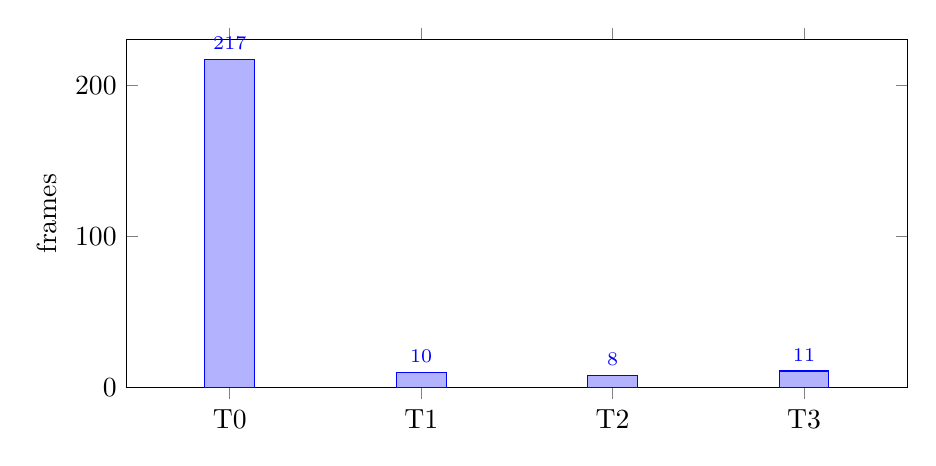
\begin{tikzpicture}
    \begin{axis}[
      ybar, bar width=18pt,
      width=11.5cm, height=6cm,
      ymin=0, ymax=230,
      symbolic x coords={T0,T1,T2,T3},
      xtick=data,
      ylabel={frames},
      nodes near coords, nodes near coords style={font=\scriptsize},
      enlarge x limits=0.18,
    ]
    \addplot coordinates {(T0,217) (T1,10) (T2,8) (T3,11)};
    \end{axis}
  \end{tikzpicture}
  \caption{Per-frame $(T,F,C)$ distribution over the $246$ candidate
    frames of R283's universe. Since $F\equiv0$ and $C=T$ (V4/V7), the
    $T$-coordinate is the whole datum; the $T{=}0$ bar is the $217$
    void frames (V1). Counts [COMPUTED]$\times2$~\cite{D289}.}
  \label{fig:tfc}
\end{figure}

\paragraph{The cell-0 gap.} The same datum resolved R285's cell-0 gap as
contingent, not structural~\cite{D289}. The $k_0=0$ impossibility is
[PROVED] (Lean \texttt{k0\_zero\_impossible}): no lane-$N$ R7 family
with $a+b=(4c-1)h$ has $k_0=0$ — at $k_0=0$, $ab\mid ch$ forces
$ab\le ch$, but $a,b\ge1$ with $a+b=(4c-1)h$ give
$ab\ge(4c-1)h-1>ch$, contradiction. Yet surgical-at-$0$ families
\emph{exist} beyond R7's discovery bounds: the flagship
$(a,b,c,h,k_0,m')=(5,553,70,2,910,2765)$ [COMPUTED]$\times2$
end-to-end, with arithmetic skeleton [PROVED] in Lean
(\url{surgical_cell0_witness}, Assumption~\ref{asm:cell0}):
$a+b=558=(4\cdot70-1)\cdot2$, $35\mid2765$,
$k_0=910\equiv0\pmod{35}$, $\mathrm{covered}=\{0\}$,
$(T,F,C)=(0,0,0)$; the ES identity $4/n=1/x+1/D_1+1/D_2$ verified at
$k=910$ ($n=21841$) and $k=3675$~\cite{D289}. The $1{,}097$-quad census
($4{,}066$ (quad,$k_0$) solutions, $ab\le200{,}000$, $h\le100$) is cited
[COMPUTED]$\times2$ but remains review-UNVERIFIED as a Lean claim
per Q-34's verdict D; ``every $k\equiv0\bmod35$'' obstruction is
[OPEN]~\cite{D289,D314}.

\subsection{Parameterized defect calculus [PROVED*]-staged}

Let $W$ be arbitrary finite, $n=|W|$ ($n=0$ allowed), $N'_W$ as
in~\eqref{eq:nprime} under componentwise union $\oplus$ (identity
$e=(\varnothing,\varnothing)$), with the defect datum~\eqref{eq:defect}.
Then $|N'_W|=\sum_{A\subseteq W}2^{|A|}=3^n$ (binomial theorem)~\cite{D300}.
The following are machine-checked but review-staged (formalization
pending — \S\ref{sec:formal}):

\begin{proposition}[P1--P2; Lean additive\_iff\_disjoint, defect\_core,
  fully\_additive\_submonoid, disjoint\_footprint\_submonoid]
  \label{prop:p}
  \begin{itemize}
  \item[P1] (defect formula)~\eqref{eq:defectop} holds for all finite
    $W$: $d$ is additive on $(x,y)$ iff $A_1\cap A_2=\varnothing$.
  \item[P2(i)] The defect-0 core $C(N'_W)=\{e\}$ for all finite $W$
    (including $W=\varnothing$).
  \item[P2(ii)] The only submonoid on which $d$ is additive on
    \emph{all} ordered pairs (including the diagonal $(x,x)$) is
    $\{e\}$: idempotence $x\oplus x=x$ gives
    $d(x)=2d(x)$, hence $d(x)=0$ — the obstruction is exactly the
    diagonal.
  \item[P2(iii)(a)] A submonoid with pairwise-disjoint footprints has at
    most one non-identity element; exactly $3^n$ such submonoids exist.
  \end{itemize}
\end{proposition}

Hand proofs are in~\cite{D300} (R59/R63-clean); the [COMPUTED]$\times2$
census (exact agreement, diff NONE) for $n=0\ldots4$ confirms the closed
forms of Table~\ref{tab:census}, and $n=3$ reproduces R296's exact
census $27/125/142/40/27/8$ as a cross-check~\cite{D300}. Classical
carve-outs (not claimed): $2^n\!\cdot\!\mathrm{Bell}(n)$ is OEIS A055882;
Bell/Stirling numbers and semilattice background are classical~\cite{D300}.

\begin{table}[t]
  \centering
  \caption{Parameterized defect-calculus closed forms [COMPUTED]$\times2$,
    $n=0\ldots4$ (R300). The $n=3$ column is R296's exact census,
    reproduced~\cite{D300}.}
  \label{tab:census}
  \begin{tabular}{llccccc}
    \toprule
    quantity & closed form & $n{=}0$ & $n{=}1$ & $n{=}2$ & $n{=}3$ & $n{=}4$ \\
    \midrule
    $|N'_W|$ & $3^n$ & $1$ & $3$ & $9$ & $27$ & $81$ \\
    additive ordered pairs & $5^n$ & $1$ & $5$ & $25$ & $125$ & $625$ \\
    disjoint-footprint families &
      $2\sum_{j=0}^n\binom{n}{j}B_j2^j$ &
      $2$ & $6$ & $26$ & $142$ & $914$ \\
    maximal families & $2^n B_n$ & $1$ & $2$ & $8$ & $40$ & $240$ \\
    pd-footprint submonoids & $3^n$ & $1$ & $3$ & $9$ & $27$ & $81$ \\
    maximal-family submonoids & $2^n$ & $1$ & $2$ & $4$ & $8$ & $16$ \\
    \bottomrule
  \end{tabular}
\end{table}

\subsection{Product theory T1/T1$'$/T2 [PROVED*]-staged}

For disjoint finite $W,V$, $U=W\sqcup V$,
\begin{equation}
  \label{eq:phipsi}
  \Phi(A,B)=\bigl((A\cap W,B\cap W),(A\cap V,B\cap V)\bigr),
\end{equation}
with inverse $\Psi((A_1,B_1),(A_2,B_2))=(A_1\cup A_2,B_1\cup B_2)$:
\emph{T1} — $\Phi:N'_U\to N'_W\times N'_V$ is a defect-preserving
monoid isomorphism (Lean \url{Phi_mul}, \url{Phi_defect},
\url{Phi_Psi}, \url{Psi_Phi}) [PROVED*]-staged~\cite{D319}.

The honest failure mode is \emph{T1$'$} (Lean
\url{Rho_mul}, \url{Rho_injective_on}, \url{Rho_defect},
\url{Rho_image_agree}) [PROVED*]-staged: for \emph{not necessarily
disjoint} $W,V$,
\begin{equation}
  \label{eq:rho}
  \rho(A,B)=\bigl((A\cap W,B\cap W),(A\cap V,B\cap V)\bigr)
\end{equation}
is a monoid homomorphism, injective on elements supported in $W\cup V$,
with image exactly the agreement-on-overlap set
($A_1\cap V=A_2\cap W$, $B_1\cap V=B_2\cap W$) — and the defect identity
carries the overlap correction
$|A\cap W|+|A\cap V|=|A|+|A\cap W\cap V|$, which vanishes exactly when
$W\cap V=\varnothing$, recovering T1~\cite{D319}.

\emph{T2} (Lean \url{prod_additive_iff}) [PROVED*]-staged: on
$N'_W\times N'_V$ with $d_\times(z)=d_W(x)+d_V(y)$,
\begin{equation}
  \label{eq:proddefect}
  d_\times(z_1\oplus z_2)=d_\times(z_1)+d_\times(z_2)
  -(\delta_W+\delta_V,\,0,\,\delta_W+\delta_V),
\end{equation}
$\delta_W=|A_1\cap A_2|$, $\delta_V=|C_1\cap C_2$: the obstruction is
additive across factors — \emph{no cross-term} — so $d_\times$ is
additive on $(z_1,z_2)$ iff additive in each factor iff footprints are
disjoint in each factor~\cite{D319}.

\subsection{Defect homomorphisms [PROVED]}

\begin{theorem}[Defect-homomorphism rigidity; Lean
  \url{defect_hom_rigidity}]
  \label{thm:h1}
  Let $W$ be finite. The only monoid homomorphism
  $f:N'_W\to M$, with $M$ an additive cancellative monoid, is the zero
  map. The same holds for $N'_W\times N'_V$ and for $(P(W),\cup)$.
\end{theorem}

\begin{proof}[Proof (R319 §4, machine-checked)]
Every $x\in N'_W$ is idempotent: $x\oplus x=x$ (componentwise union).
For a homomorphism $f$,
\begin{equation}
  \label{eq:h1}
  f(x)=f(x\oplus x)=f(x)+f(x)=2f(x),
\end{equation}
and $M$ cancellative gives $f(x)=0$ for all $x$. Q-58's nits are
honored: no ``$W$ finite'' or $k\ge1$ hypothesis is needed ($W=\varnothing$
gives $N'_\varnothing=\{e\}$, trivial; $k=0$ vacuous)~\cite{D319,D322}.
\end{proof}

Q-45/Q-58 record H1 as \emph{classical} (the idempotent-collapse lemma
for semilattices to abelian groups), not a novelty claim~\cite{D291,D322}.
No tension with H3 (defect-exact classification, gate-passed, owed to
the dedicated lane): H3 classifies maps with
``$f(x\oplus y)=f(x)+f(y)\iff$ disjoint footprints'' — a different
hypothesis — which exist nontrivially~\cite{D319}.

\begin{theorem}[Split boundary; Lean \url{split_boundary_witness}]
  \label{thm:c1}
  For finite disjoint $W,V$: every maximal defect-additive family of
  $N'_W\times N'_V$ splits (no block meets both factors) iff $W=\varnothing$
  or $V=\varnothing$ [PROVED*].
\end{theorem}

The $(\Leftarrow)$ direction is vacuous; $(\Rightarrow)$ uses the mixed
witness $F^\star=\{(1,1),((W,\varnothing),(V,\varnothing))\}$: for
nonempty $W,V$ this is the single-block maximal family whose unique
block meets both factors (maximality via the P2(iv) classification,
staged) — [PROVED] in Lean as the witness inequality
$(1,1)\ne((W,\varnothing),(V,\varnothing))$~\cite{D319,D322}.

\begin{corollary}[Mixed counts; Lean \url{mixed_count},
  \texttt{mixed\_count\_11/21/22}]
  \label{cor:c2}
  The identity $\#\mathrm{mixed}=\#\mathrm{total}-\#\mathrm{split}$
  (total$=2^{n+m}\mathrm{Bell}(n+m)$ via T3, split$=2^{n+m}
  \mathrm{Bell}(n)\mathrm{Bell}(m)$ via T4, gate-passed [PROVED*]) is
  [PROVED] in Lean, with the concrete values
  \begin{equation}
    \label{eq:mixedcount}
    (1,1){:}\ 4,\qquad (2,1){:}\ 24,\qquad (2,2){:}\ 176,
  \end{equation}
  all nonzero — ``all maximal families split'' is REFUTED.
\end{corollary}

The numbers~\eqref{eq:mixedcount} are [COMPUTED]$\times2$
($r319$\_\allowbreak split\_path$1/2$, exact agreement; maximality
re-verified per family)~\cite{D319}. The smallest explicit witness
(both JSONs; ``a smallest'', four equally small at $(1,1)$ per Q-58) is
$W=\{0\}$, $V=\{1\}$, blocks $[[0,1]]$, family
$\{(\varnothing,\varnothing),(\{0,1\},\varnothing)\}$~\cite{D319}.
Record correction C3 (Q-58 $\checkmark$): the four maximal-family submonoids at
$(1,1)$ are the single-block families — all \emph{mixed}, not split;
$(1,1)$ is $8$ maximal $=4$ split $+4$ mixed~\cite{D319,D322}.
Figure~\ref{fig:split} shows the decomposition.

\begin{figure}[t]
  \centering
  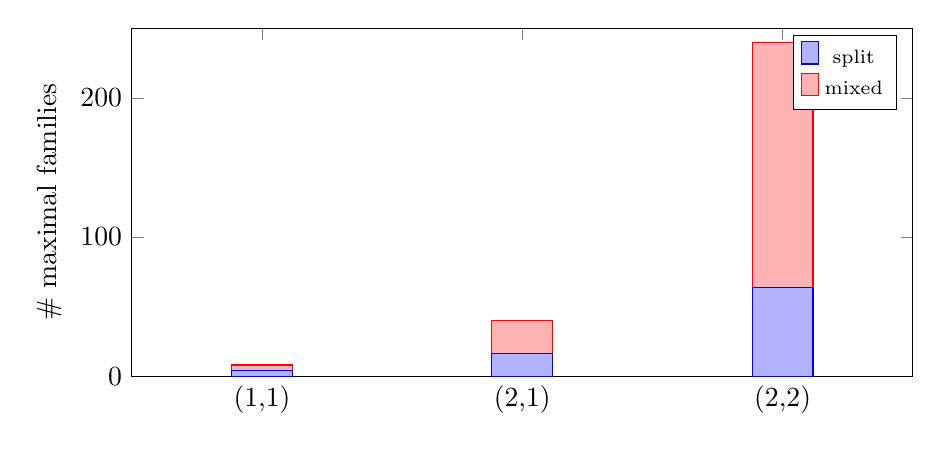
\begin{tikzpicture}
    \begin{axis}[
      ybar stacked, bar width=22pt,
      width=11.5cm, height=6cm,
      ymin=0, ymax=250,
      symbolic x coords={{(1{,}1)},{(2{,}1)},{(2{,}2)}},
      xtick=data,
      ylabel={\# maximal families},
      legend style={at={(0.98,0.98)},anchor=north east,font=\scriptsize},
      enlarge x limits=0.25,
    ]
    \addplot coordinates {({(1{,}1)},4) ({(2{,}1)},16) ({(2{,}2)},64)};
    \addplot coordinates {({(1{,}1)},4) ({(2{,}1)},24) ({(2{,}2)},176)};
    \legend{split,mixed}
    \end{axis}
  \end{tikzpicture}
  \caption{Maximal defect-additive families: split vs mixed (stacked),
    totals $8/40/240$ at $(n,m)=(1,1),(2,1),(2,2)$. The mixed bar
    refutes ``all maximal families split'' (C1/C2). Counts
    [COMPUTED]$\times2$~\cite{D319}.}
  \label{fig:split}
\end{figure}

\begin{theorem}[Literal products never work; Lean
  \url{literal_product_never}]
  \label{thm:c4}
  No literal product $F_W\times F_V$ of nontrivial families is
  defect-additive.
\end{theorem}

\begin{proof}[Proof (R319 §5, machine-checked)]
Take $(a,b)\ne e$ in $F_W$ and $(c,d)\ne e$ in $F_V$ (both exist for
nontrivial factors). Then $z_1=(a,1)$ and $z_2=(a,c)$ are both in the
product, distinct, with $W$-footprints both $a.A$ overlapping in
$a.A\ne\varnothing$ ($a\ne e$ and $B\subseteq A$ force $a.A\ne\varnothing$,
Lean \url{idem_ne_one_imp_A_ne_empty}) — violating
\url{ProdDefectAdditive}~\cite{D319}.
\end{proof}

Q-58 verified the hypotheses airtight ($e$ in every maximal factor by
the Q-42 Submonoid convention; $a\ne\varnothing$ airtight) and checked
$(1,1)$ exhaustively: $0$ nontrivial products defect-additive among
$4$ factor pairs~\cite{D322}.

\subsection{D2(c) repair and maximal-family tiling [PROVED]}

\begin{theorem}[D2(c) repair; Lean \url{d2c_not_closed},
  \url{d2c_generated_loses_disjoint}]
  \label{thm:d2c}
  A pairwise-disjoint-footprint family with $\ge2$ non-identity elements
  is not closed under union; its generated submonoid
  $\mathrm{Submonoid.closure}\,\uparrow F$ is a submonoid by
  construction but loses pairwise disjointness.
\end{theorem}

This is the verbatim Q-39 repair (Bunny's wording, applied to the
R296 draft whose ``does NOT form a nontrivial submonoid'' was
objected): the witness $x=(\{2\},\varnothing)$,
$y=(\{3\},\varnothing)$ has disjoint footprints with
$x\oplus y=(\{2,3\},\varnothing)$ overlapping $x$'s; the $88$
pairwise-disjoint families with $\ge2$ non-identity elements are all
unclosed, all $88$ generated submonoids are submonoids losing
disjointness [COMPUTED]$\times2$ corroborating~\cite{D296,D299}.
The $26$ two-element submonoids $\{( \varnothing,\varnothing),x\}$ close
by idempotence — off-diagonal additivity is compatible with
submonoids; the diagonal pair $(x,x)$ forces $d(x)=2d(x)$ and kills
everything but $e$~\cite{D296}.

\begin{theorem}[Maximal-family tiling; Lean \url{maximal_family_tiles}]
  \label{thm:tiles}
  An inclusion-maximal pairwise-disjoint-footprint family contains the
  identity and its footprints cover every tag.
\end{theorem}

The structural core of D3: if $\bigcup A_i\ne W$, some
$w\in W\setminus\bigcup A_i$ exists and $(\{w\},\varnothing)$ strictly
extends the family~\cite{D296}. The $40/8$ census counts for
$W=\{2,3,4\}$ stay [COMPUTED]$\times2$ (cited, not formalized — no
half-formalization)~\cite{D296,D318}.

%======================================================================
\section{Discussion}
\label{sec:disc}
%======================================================================

\paragraph{Significance.} The void-frame theory is the program's
forcing framework stripped to its algebra: frames fire or they do not;
the void frames are the identity; the defect datum measures exactly how
far a product is from being a homomorphism; and H1 says no nonzero
additive measurement of the defect monoid exists at all. The surprise is
not the rigidity (it is classical idempotent-collapse) but that the
parameterized calculus closes exactly: $3^n$, $5^n$,
$2^n\!\cdot\!\mathrm{Bell}(n)$ with zero violations across two
independent code paths~\cite{D300}. The C1/C2 result is the honest
counterpoint: maximality does not imply splitting — a distributional
fact (Figure~\ref{fig:split}) the Lean witness pins exactly.

\paragraph{Novelty.} All objects are program-invented (void frames,
$(T,F,C)$, $N'$, $d$); novelty is narrow: first statements about these
objects. Classical carve-outs are stated: M2/H1 idempotent-collapse
~\cite{D291,D322}; semilattice $=$ idempotent commutative
monoid~\cite{D296}; $2^n\!\cdot\!\mathrm{Bell}(n)=$ OEIS A055882
(recorded, not claimed)~\cite{D300}; Bell/Stirling numbers. No blanket
algebraic novelty is claimed. Web-checks (2026-10-11) found no ``void
frame''/``defect-additive monoid''/``void monoid'' in the literature
(hits are unrelated: programming monoids, valuation-theory defect,
intersecting families)~\cite{D291,D296,D300}.

\paragraph{Limitations.} (i) The $217/246$ void census and all pair
censuses are [COMPUTED]$\times2$, not Lean-formalized: the machine
checks the theorems about the datum, not the census itself (no
half-formalization)~\cite{D314,D318}. (ii) Q-34's scoped verdict
explicitly withholds: the $1{,}097$-quad cell-0 census as a Lean claim,
code independence, ``every $k\equiv0\bmod35$'', and full R7 acceptance —
these are UNVERIFIED/OPEN, not proved here~\cite{D314}. (iii) The
\url{VoidMonoidParam} theorems are review-staged (build-clean,
gate-passed, Q-42/Q-45 SURVIVES, promotion pending); T3/T4/H3
formalization is owed to a dedicated lane~\cite{D314,D318}.
(iv) Beyond the exclusion lemma, void-ness is contingent edge data
([HEURISTIC]-leaning); no further structural restriction was
found~\cite{D283}. (v) The $X$-side enlargement ($X\ne A^\star$, $\tau$
not forced) is a different object class, unexamined [OPEN]~\cite{D283}.

%======================================================================
\section{Conclusion}
%======================================================================

Void frames, abundant in the swept universe ($217/246$), are the union
identity of the frame algebra and exactly the zero triple of the
$(T,F,C)$ datum (V1--V8) [PROVED]. The void-frame monoid $N'_W$ carries
an exact defect calculus: the defect formula~\eqref{eq:defectop},
parameterized closed forms (P1--P2) [PROVED*]-staged, and the
product defect-split with its honest overlap correction (T1/T1$'$/T2)
[PROVED*]-staged. The defect homomorphism theory is rigid: the only
homomorphism to a cancellative target is zero (H1) [PROVED]; literal
products of nontrivial families are never defect-additive (C4)
[PROVED]; and maximal families need not split — the mixed ones are
counted exactly (C1/C2) [PROVED*/COMPUTED]. The pairwise-disjoint
repair theorem and the maximal-family tiling theorem are [PROVED].
Everything machine-checked is formalized in Lean~4.34.1 + Mathlib
v4.34.1 with zero sorrys and standard axioms only; every census is
cited [COMPUTED] data, never called a proof. The natural next steps are
the owed formalizations (P2(iii)(b), P2(iv), T3/T4/H3), the $X$-side
void theory, and the $k\equiv0\bmod35$ general obstruction.

%======================================================================
\section{References}
%======================================================================

\begin{thebibliography}{9}

\bibitem{D280}
D.~Blair,
\emph{Unsolved Math --- Round 280: abstract lock theory [PROVED*]},
program dossier, 2026-10-11.
(Supplied datum: abstract lock frame, Theorems 1--4, 472-frame census.)

\bibitem{D283}
D.~Blair,
\emph{Unsolved Math --- Round 283: void locks --- the abstract prediction
realized; void-exclusion lemma [PROVED*]; void census [COMPUTED]$\times2$},
program dossier, 2026-10-10.
(Supplied datum: void-search universe, $217/246$ void census,
pattern census, Void-Exclusion Lemma, representative void frames.)

\bibitem{D289}
D.~Blair,
\emph{Unsolved Math --- Round 289: void frames under union forcing
(R283 $\times$ R285 cross) + the cell-0 gap CLOSED},
program dossier, 2026-10-11.
(Supplied datum: $(T,F,C)=(|u|,0,|u|)$ datum, V1--V8, $30{,}381$-pair
census, $k_0=0$ impossibility, flagship $(5,553,70,2,910,2765)$
cell-0 family, $1{,}097$-quad census, Q-34 scope notes.)

\bibitem{D291}
D.~Blair,
\emph{Unsolved Math --- Round 291: the void-frame algebra (void monoid)},
program dossier, 2026-10-11.
(Supplied datum: $N'$, $\iota$, $d$, $\pi_1/\pi_2$, S1/M1/M2/M3/X1/X2/F1,
E/C/V classes, $60{,}516$-pair census.)

\bibitem{D296}
D.~Blair,
\emph{Unsolved Math --- Round 296: defect core of the void-frame monoid},
program dossier, 2026-10-11.
(Supplied datum: D1/D2/D3, $27$-submonoid classification, $40$-family
census, draft-error log.)

\bibitem{D299}
D.~Blair,
\emph{Unsolved Math --- Round 299: D2(c) wording repair (Q-39)},
program dossier, 2026-10-11.
(Supplied datum: verbatim Q-39 repair, $88$-family re-verification.)

\bibitem{D300}
D.~Blair,
\emph{Unsolved Math --- Round 300: parameterized defect calculus},
program dossier, 2026-10-11.
(Supplied datum: $N'_W$ parameterized, P1, P2(i)--(iv), closed forms,
$n=0\ldots4$ census, Q-42 gate.)

\bibitem{D314}
D.~Blair,
\emph{Unsolved Math --- Round 314: Lean + rule-9 lane},
program dossier, 2026-10-11.
(Supplied datum: \url{VoidMonoidParam.lean} fold record, Q-42/Q-45
SURVIVES, R314 build gate, Q-34 scope notes, owed-formalization list.)

\bibitem{D318}
D.~Blair,
\emph{Unsolved Math --- Round 318: Lean + rule-9 lane},
program dossier, 2026-10-11.
(Supplied datum: \url{VoidMonoid.lean} fold record
(\url{d2c_not_closed}, \url{d2c_generated_loses_disjoint},
\url{maximal_family_tiles}), R318 build gate, owed-T3/T4/H3 note.)

\bibitem{D319}
D.~Blair,
\emph{Unsolved Math --- Round 319: R303 product-defect theory filed +
maximal splitting classification},
program dossier, 2026-10-11.
(Supplied datum: T1/T1$'$/T2 hand proofs, H1 hand proof, C1 split
boundary, C2 mixed counts $(1,1){:}\,4$, $(2,1){:}\,24$, $(2,2){:}\,176$,
C3 record correction, C4 literal-product theorem.)

\bibitem{D322}
D.~Blair,
\emph{Unsolved Math --- Round 322: Lean + rule-9 lane},
program dossier, 2026-10-11.
(Supplied datum: \url{VoidDefectHom.lean} fold record
(\url{defect_hom_rigidity}, \url{literal_product_never},
\url{split_boundary_witness}, \url{mixed_count}), Q-58
SURVIVES, $34$-theorem batch gate, axiom audit.)

\bibitem{D310}
D.~Blair,
\emph{Unsolved Math --- Round 310: Lean + rule-9 lane},
program dossier, 2026-10-11.
(Supplied datum: bakkie full-library build gate, exit~0, $17{,}936$
jobs, axiom audit, [PROVED] promotions of VoidLock/VoidUnion.)

\end{thebibliography}

\end{document}

% --- Author self-review: SUBSTANTIVE WEAKNESSES (must fix before submission) ---
% 1. The parameterized census table (Tab.~\ref{tab:census}) states the P2(iv)
%    count $2^n\cdot\mathrm{Bell}(n)$ and the pd-submonoid count $3^n$ as
%    "closed forms" but the paper presents only P2(i)-(iii)(a) as theorems;
%    P2(iii)(b) and P2(iv) are formalization-owed and should not sit in the
%    same table without their staged-label carried on every row. The table
%    caption cites [COMPUTED]x2, but a reader will reasonably read the closed
%    forms as theorems — the row-level honesty labels need to move into the
%    table itself (e.g. a status column), not just the surrounding prose.
% 2. H1 (Theorem~\ref{thm:h1}) is recorded as "classical, not a novelty claim"
%    yet occupies full proof-claiming theorem space identical in weight to the
%    genuinely new C1/C2/C4 results. The paper should either downgrade H1 to
%    a Lemma/Remark (it's a two-line idempotence argument) or add a sentence
%    explaining why its formalization matters despite being classical (it is
%    the rigidity premise C1-C4 all quietly rely on).
% 3. The cell-0 flagship $(5,553,70,2,910,2765)$ is carried through R289's
%    (T,F,C) datum $(0,0,0)$ into a paper whose title promises defect calculus,
%    but its connection to $N'$ and $d$ is never made explicit — it is a
%    $(T,F,C)$-datum object (pc families), not an $N'$-object, and the paper
%    quietly conflates the two readings of the triple. A bridging sentence
%    (or its deletion from this paper) is needed.
% --- Author self-review: TYPOGRAPHY ISSUES ---
% 1. The theorem-environment label "(V1)" etc. inside itemize uses \item[V1]
%    with a colon convention inconsistent with the named-theorem style
%    "[Lean ...]" used elsewhere; the V1-V8 items should use a uniform
%    label scheme (e.g. bold tags matching the Lean names) so cross-references
%    (\ref) don't dangle — currently only the Proposition itself is labeled.
% 2. The pgfplots ybar-stacked legend sits at the plot's north-east corner
%    over the tallest bar's top region at ymax=250; if a later data revision
%    pushes the (2,2) mixed bar higher, the legend will overlap the bar.
%    Anchor it outside (legend pos=north west or legend to name) instead.
% 3. Table~\ref{tab:formal} spans nearly full page width and will likely
%    produce an overfull \hbox in 11pt/a4 with 2.5cm margins because the
%    Lean-name columns are unbreakable; consider \small font or \tabularx
%    with breakable identifier columns.
